\documentclass{standalone}
\usepackage{tikz}
\usetikzlibrary{patterns, positioning}


\begin{document}
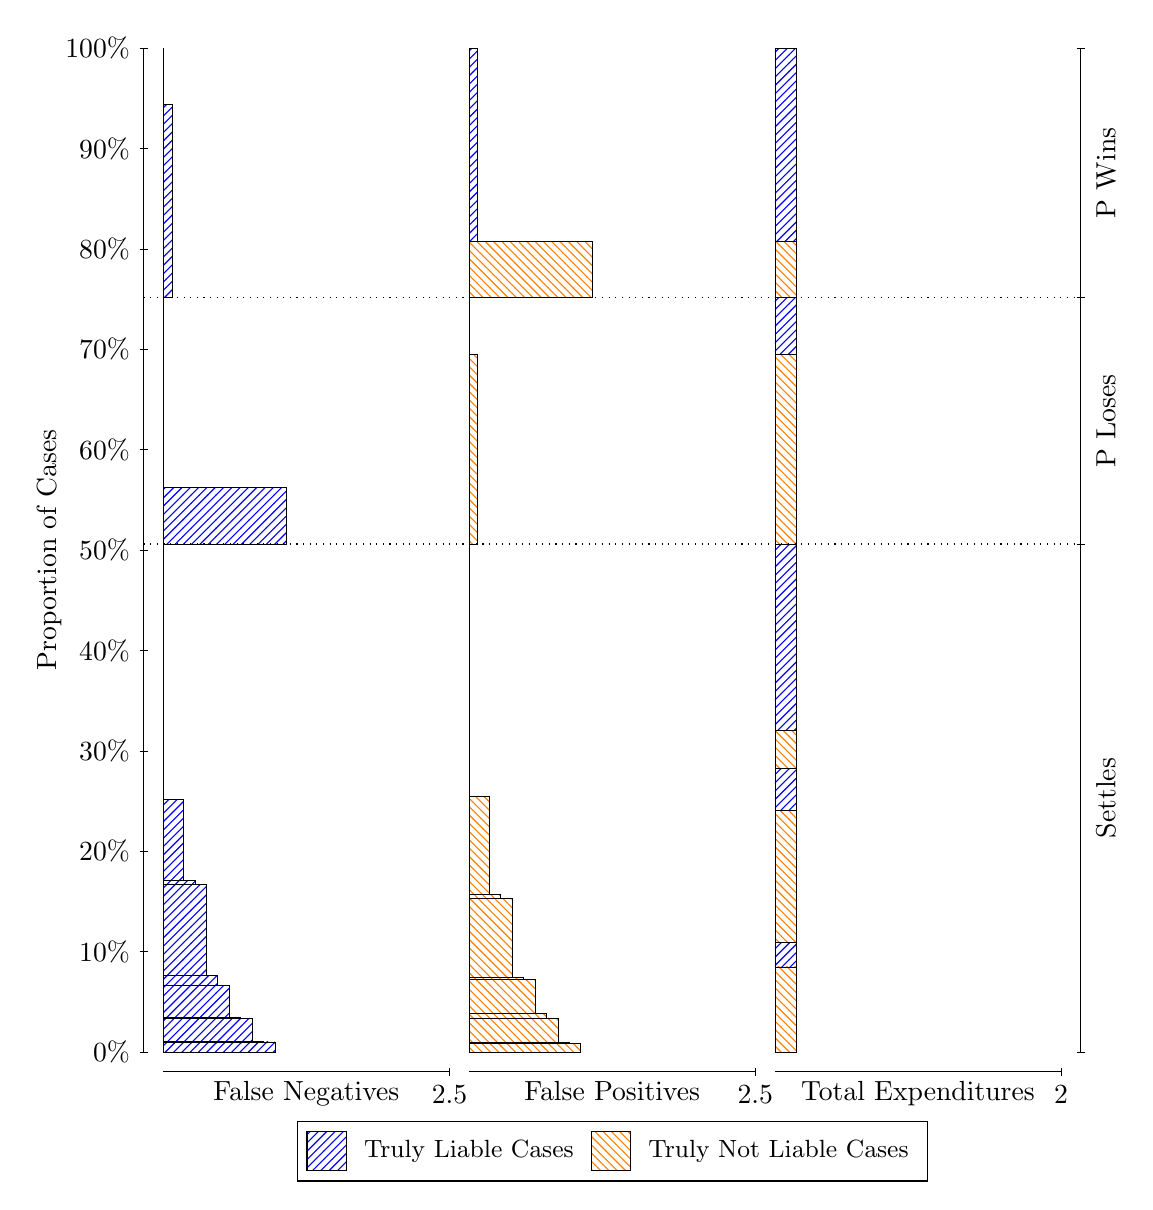
\begin{tikzpicture}
\draw[black, very thin] (1.5,1.75) -- (1.5,14.5);
\node[rotate=90, text=black, anchor=center] at (0.3, 8.125) {Proportion of Cases};
\draw[black, very thin] (1.45,1.75) -- (1.55,1.75);
\node[text=black, anchor=east] at (1.45, 1.75) {0\%};
\draw[black, very thin] (1.45,3.025) -- (1.55,3.025);
\node[text=black, anchor=east] at (1.45, 3.025) {10\%};
\draw[black, very thin] (1.45,4.3) -- (1.55,4.3);
\node[text=black, anchor=east] at (1.45, 4.3) {20\%};
\draw[black, very thin] (1.45,5.575) -- (1.55,5.575);
\node[text=black, anchor=east] at (1.45, 5.575) {30\%};
\draw[black, very thin] (1.45,6.85) -- (1.55,6.85);
\node[text=black, anchor=east] at (1.45, 6.85) {40\%};
\draw[black, very thin] (1.45,8.125) -- (1.55,8.125);
\node[text=black, anchor=east] at (1.45, 8.125) {50\%};
\draw[black, very thin] (1.45,9.4) -- (1.55,9.4);
\node[text=black, anchor=east] at (1.45, 9.4) {60\%};
\draw[black, very thin] (1.45,10.675) -- (1.55,10.675);
\node[text=black, anchor=east] at (1.45, 10.675) {70\%};
\draw[black, very thin] (1.45,11.95) -- (1.55,11.95);
\node[text=black, anchor=east] at (1.45, 11.95) {80\%};
\draw[black, very thin] (1.45,13.225) -- (1.55,13.225);
\node[text=black, anchor=east] at (1.45, 13.225) {90\%};
\draw[black, very thin] (1.45,14.5) -- (1.55,14.5);
\node[text=black, anchor=east] at (1.45, 14.5) {100\%};

\draw[black, very thin] (13.4,1.75) -- (13.4,14.5);
\draw[black, very thin] (13.35,1.75) -- (13.45,1.75);
\node[anchor=west] at (13.35, 1.75) {};
\draw[black, very thin] (13.35,8.2011) -- (13.45,8.2011);
\node[anchor=west] at (13.35, 8.2011) {};
\draw[black, very thin] (13.35,11.329) -- (13.45,11.329);
\node[anchor=west] at (13.35, 11.329) {};
\draw[black, very thin] (13.35,14.5) -- (13.45,14.5);
\node[anchor=west] at (13.35, 14.5) {};

\draw[black, very thin, pattern color=blue, pattern=north east lines] (1.75,1.75) rectangle (3.167,1.8791);
\draw[black, very thin, pattern color=blue, pattern=north east lines] (1.75,1.8791) rectangle (3.0217,1.8886);
\draw[black, very thin, pattern color=blue, pattern=north east lines] (1.75,1.8886) rectangle (2.8763,2.173);
\draw[black, very thin, pattern color=blue, pattern=north east lines] (1.75,2.173) rectangle (2.731,2.1863);
\draw[black, very thin, pattern color=blue, pattern=north east lines] (1.75,2.1863) rectangle (2.5857,2.5917);
\draw[black, very thin, pattern color=blue, pattern=north east lines] (1.75,2.5917) rectangle (2.4403,2.7221);
\draw[black, very thin, pattern color=blue, pattern=north east lines] (1.75,2.7221) rectangle (2.295,3.88);
\draw[black, very thin, pattern color=blue, pattern=north east lines] (1.75,3.88) rectangle (2.1497,3.9291);
\draw[black, very thin, pattern color=blue, pattern=north east lines] (1.75,3.9291) rectangle (2.0043,4.9546);
\draw[black, very thin, pattern color=orange, pattern=north west lines] (1.75,4.9546) rectangle (1.75,8.2011);
\draw[black, very thin, pattern color=blue, pattern=north east lines] (1.75,8.2011) rectangle (3.3123,8.9184);
\draw[black, very thin, pattern color=orange, pattern=north west lines] (1.75,8.9184) rectangle (1.75,11.329);
\draw[black, very thin, pattern color=blue, pattern=north east lines] (1.75,11.329) rectangle (1.859,13.782);
\draw[black, very thin, pattern color=orange, pattern=north west lines] (1.75,13.782) rectangle (1.75,14.5);
\draw[black, very thin, pattern color=orange, pattern=north west lines] (5.6333,1.75) rectangle (7.0503,1.8604);
\draw[black, very thin, pattern color=orange, pattern=north west lines] (5.6333,1.8604) rectangle (6.905,1.8699);
\draw[black, very thin, pattern color=orange, pattern=north west lines] (5.6333,1.8699) rectangle (6.7597,2.1763);
\draw[black, very thin, pattern color=orange, pattern=north west lines] (5.6333,2.1763) rectangle (6.6143,2.2366);
\draw[black, very thin, pattern color=orange, pattern=north west lines] (5.6333,2.2366) rectangle (6.469,2.6698);
\draw[black, very thin, pattern color=orange, pattern=north west lines] (5.6333,2.6698) rectangle (6.3237,2.6963);
\draw[black, very thin, pattern color=orange, pattern=north west lines] (5.6333,2.6963) rectangle (6.1783,3.7024);
\draw[black, very thin, pattern color=orange, pattern=north west lines] (5.6333,3.7024) rectangle (6.033,3.7515);
\draw[black, very thin, pattern color=orange, pattern=north west lines] (5.6333,3.7515) rectangle (5.8877,4.9964);
\draw[black, very thin, pattern color=blue, pattern=north east lines] (5.6333,4.9964) rectangle (5.6333,8.2011);
\draw[black, very thin, pattern color=orange, pattern=north west lines] (5.6333,8.2011) rectangle (5.7423,10.612);
\draw[black, very thin, pattern color=blue, pattern=north east lines] (5.6333,10.612) rectangle (5.6333,11.329);
\draw[black, very thin, pattern color=orange, pattern=north west lines] (5.6333,11.329) rectangle (7.1957,12.047);
\draw[black, very thin, pattern color=blue, pattern=north east lines] (5.6333,12.047) rectangle (5.7423,14.5);
\draw[black, very thin, pattern color=orange, pattern=north west lines] (9.5167,1.75) rectangle (9.7892,2.8317);
\draw[black, very thin, pattern color=blue, pattern=north east lines] (9.5167,2.8317) rectangle (9.7892,3.1389);
\draw[black, very thin, pattern color=orange, pattern=north west lines] (9.5167,3.1389) rectangle (9.7892,4.8171);
\draw[black, very thin, pattern color=blue, pattern=north east lines] (9.5167,4.8171) rectangle (9.7892,5.3515);
\draw[black, very thin, pattern color=orange, pattern=north west lines] (9.5167,5.3515) rectangle (9.7892,5.8381);
\draw[black, very thin, pattern color=blue, pattern=north east lines] (9.5167,5.8381) rectangle (9.7892,8.2011);
\draw[black, very thin, pattern color=orange, pattern=north west lines] (9.5167,8.2011) rectangle (9.7892,10.612);
\draw[black, very thin, pattern color=blue, pattern=north east lines] (9.5167,10.612) rectangle (9.7892,11.329);
\draw[black, very thin, pattern color=orange, pattern=north west lines] (9.5167,11.329) rectangle (9.7892,12.047);
\draw[black, very thin, pattern color=blue, pattern=north east lines] (9.5167,12.047) rectangle (9.7892,14.5);
\draw[black, dotted] (1.5,8.2011) -- (13.4,8.2011);
\draw[black, dotted] (1.5,11.329) -- (13.4,11.329);
\draw[black, very thin] (1.75,1.5) -- (5.3833,1.5);
\node[text=black, anchor=north] at (3.5667, 1.5) {False Negatives};
\draw[black, very thin] (5.3833,1.45) -- (5.3833,1.55);
\node[text=black, anchor=north] at (5.3833, 1.45) {2.5};

\draw[black, very thin] (5.6333,1.5) -- (9.2667,1.5);
\node[text=black, anchor=north] at (7.45, 1.5) {False Positives};
\draw[black, very thin] (9.2667,1.45) -- (9.2667,1.55);
\node[text=black, anchor=north] at (9.2667, 1.45) {2.5};

\draw[black, very thin] (9.5167,1.5) -- (13.15,1.5);
\node[text=black, anchor=north] at (11.333, 1.5) {Total Expenditures};
\draw[black, very thin] (13.15,1.45) -- (13.15,1.55);
\node[text=black, anchor=north] at (13.15, 1.45) {2};

\node[text=black, centered, rotate=90] at (13.72, 4.9755) {Settles};
\node[text=black, centered, rotate=90] at (13.72, 9.7651) {P Loses};
\node[text=black, centered, rotate=90] at (13.72, 12.915) {P Wins};

\draw (7.449999999999999,1.5) node[draw=none] (baseCoordinate) {};
\begin{scope}[align=center]
        \matrix[scale=0.5, draw=black, below=0.5cm of baseCoordinate, nodes={draw}, column sep=0.1cm]{
            \node[rectangle, draw, minimum width=0.5cm, minimum height=0.5cm, pattern color=blue, pattern=north east lines] {}; &
            \node[draw=none, font=\small, text=black] (B) {Truly Liable Cases}; &
            \node[rectangle, draw, minimum width=0.5cm, minimum height=0.5cm, pattern color=orange, pattern=north west lines] {}; &
            \node[draw=none, font=\small, text=black] (B) {Truly Not Liable Cases}; \\
            };
\end{scope}

\end{tikzpicture}
\end{document}